\documentclass{article}
\usepackage{tikz}

\definecolor{OliveGreen}{RGB}{85, 107, 47}
\definecolor{RoyalPurple}{RGB}{120, 81, 169}
\definecolor{NavyBlue}{RGB}{0, 0, 128}
\definecolor{CornflowerBlue}{RGB}{100, 149, 237}
\definecolor{Cerulean}{RGB}{0, 123, 167}
\definecolor{DarkOrchid}{RGB}{153, 50, 204}

\begin{document}

\section*{No Derivative}
\begin{minipage}[h]{0.7\textwidth}
  \centering
  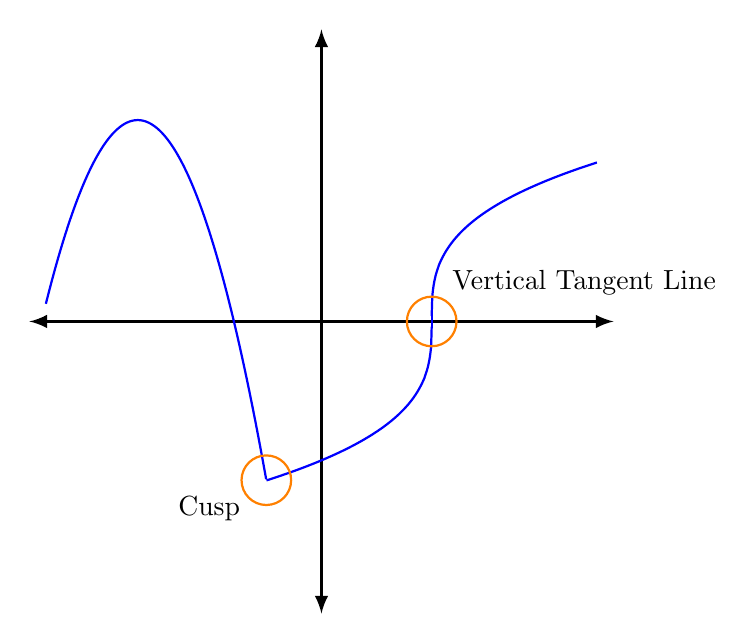
\begin{tikzpicture}[scale=0.7]
    \draw[latex-latex, very thick] (-5.3,0)--(5.3,0);
    \draw[latex-latex, very thick] (0,-5.3)--(0,5.3);
  
    \draw[domain=2.0001:5,samples=300,smooth,variable=\x, blue,  thick] plot ({\x},{2*exp(ln(\x-2)/3)});
    \draw[domain=2.0001:5,samples=300,smooth,variable=\x, blue,  thick,rotate around={180:(2,0)}] plot ({\x},{2*exp(ln(\x-2)/3)});
    \draw[blue,thick] (2,-0.1)--(2,0.1);
    \draw[domain=-5:-1,samples=300,smooth,variable=\x, blue,  thick] plot ({\x},-1.2*\x*\x-8*\x-9.68);
    \draw[orange,thick](-1,-2.88) circle (0.45);
    \draw[orange,thick](2,0) circle (0.45);
    \node[left] at (-1.3,-3.4) {Cusp};
    \node[above right] at (2.2,0.3) {Vertical Tangent Line};
  \end{tikzpicture}
\end{minipage}%
\begin{minipage}[t]{0.5\textwidth}
This graph represents a function that is not differentiable at certain points. The presence of a cusp and vertical tangent lines indicates that the function lacks a derivative at those points.
\end{minipage}

\section*{Inverse Derivative}
\begin{minipage}[h]{0.7\textwidth}
  \centering
  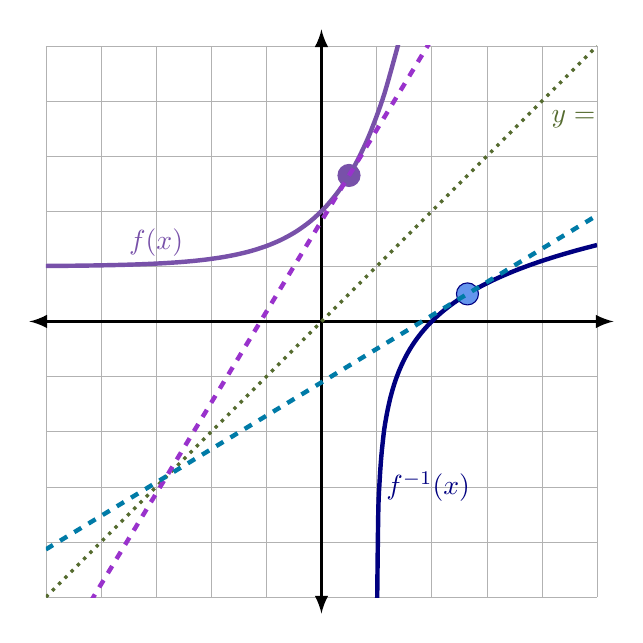
\begin{tikzpicture}[scale=0.7]
    \draw[black!30!white, very thin] (-5,-5) grid (5,5);
    \draw[latex-latex, very thick] (-5.3,0)--(5.3,0);
    \draw[latex-latex, very thick] (0,-5.3)--(0,5.3);
    
    \begin{scope}
        \clip (-5,-5) rectangle (5,5);
        \draw[very thick, OliveGreen,dotted](-5,-5)--(5,5);
        \node[OliveGreen,below right] at (4,4) {$y=x$};
        
        \draw[domain=-5:1.4,smooth,variable=\x, RoyalPurple, ultra thick] plot ({\x},{exp(\x)+1});
        \node[RoyalPurple,above] at (-3,1) {$f(x)$};
        \draw[RoyalPurple,fill=RoyalPurple] (0.5,2.649) circle [radius=0.2];
        \draw[domain=-4.5:2,smooth,variable=\x, DarkOrchid, ultra thick,dashed] plot ({\x},{1.649*\x+1.824});
        
        \draw[domain=1.003:5,smooth,variable=\x, NavyBlue, ultra thick, samples=150] plot ({\x},{ln(\x-1)});
        \node[NavyBlue,right] at (1,-3) {$f^{-1}(x)$};
        \draw[NavyBlue,fill=CornflowerBlue] (2.649,0.5) circle [radius=0.2];
        \draw[domain=-5:5,smooth,variable=\x, Cerulean, ultra thick,dashed] plot ({\x},{0.606*\x-1.105});
    \end{scope}
  \end{tikzpicture}
\end{minipage}%
  \vspace{2em}
\begin{minipage}[h]{0.5\textwidth}
This graph represents the inverse function of a function that has a derivative. The presence of a straight line indicates that the inverse function is linear. Additionally, the graph illustrates that the inverse function reverses the behavior of the original function with respect to the line $y=x$.
\end{minipage}

\end{document}
